\documentclass[a4paper,12pt]{report}

\usepackage[a4paper,left=2cm,right=2cm,top=2cm,bottom=2cm]{geometry}
\usepackage[pdftex]{graphicx,color}
\usepackage[utf8]{inputenc}
\usepackage[brazil]{babel}
\usepackage{url}
\usepackage[T1]{fontenc}
\usepackage{amsmath,amssymb,amsfonts,textcomp}
\usepackage{color}
\usepackage{fancyhdr}
\usepackage{fancyvrb}
\usepackage{multirow}
\usepackage{textfit}
\usepackage{rotating}
\usepackage{setspace}
\usepackage{subfigure}
\usepackage{listings}
\usepackage{abntex2cite}
\usepackage{float}
\usepackage[dvipdfm]{hyperref}% permite configurar hiperef
\hypersetup{colorlinks=true,linkcolor=blue,citecolor=blue}
% \hypersetup{
% pdftitle = {Revisão Bibliografica},
% pdfsubject = {SMA*},
% pdfkeywords = {ODPA,PDF,PS,OSI,RMI,BGP,Q-learning},
% pdfauthor = {Michell Stuttgart Faria}
% }

\lstset{
   numbers=left, % Numeros ao lado esquerdo do algoritmo
   stepnumber=1, % Incremento
   firstnumber=1, % Inicio
   numberstyle=\footnotesize\textit, % Estilo da fonte
   extendedchars=true,
   breaklines=true,
   frame=tb,
   basicstyle=\footnotesize,
   stringstyle=\ttfamily,
   showstringspaces=false,
   keywordstyle=\color[rgb]{0,0,1},
   commentstyle=\color[rgb]{0.133,0.545,0.133},
   stringstyle=\color[rgb]{0.627,0.126,0.941}
}

\newcommand{\ingles}{\foreignlanguage{english}}

\begin{document}

% _________________________ Capa __________________________

\begin{titlepage}

\begin{table}[!ht]

\begin{doublespacing}

  \begin{tabular}{c c}
      \multirow{4}{*} { 
\includegraphics[height=2.7cm]{brasao.pdf}  }
      & \multicolumn{1}{c}{ } \\
      & \multicolumn{1}{c}{ \LARGE{\textbf{Instituto de Engenharia de Sistemas e }} } \\
      & \multicolumn{1}{c}{ \LARGE{\textbf{Tecnologias da Informação (IESTI)}} } \\
      & \multicolumn{1}{c}{ } \\

      \multirow{6}{*}{ \rotatebox{90}{ \Huge{\textbf{Universidade Federal de Itajubá} } } }
      & \multicolumn{1}{c}{ \vspace{1cm} } \\     
      & \begin{tabular}{| c |}
          \hline
              \Large{\textbf{SAGA Game Library}} \\
              \Large{\textbf{Biblioteca para desenvolvimento}} \\
              \Large{\textbf{de jogos eletrônicos}} \\

          \hline
        \end{tabular} \\
      
      & \multicolumn{1}{c}{ \vspace{1cm} } \\     
      & \begin{tabular}{ c }
              \Large{\textbf{TRABALHO FINAL}} \\
              \Large{\textbf{DO CURSO DE}} \\
              \Large{\textbf{ENGENHARIA DA COMPUTAÇÃO}} \\
        \end{tabular} \\
        
      & \multicolumn{1}{c}{ \vspace{1cm} } \\     
      & \begin{tabular}{| l |}
          \hline
              \Large{\textbf{Aluno: Alfredo José de Paula Barbosa - 16890}} \\
              \Large{\textbf{Aluno: Michell Stuttgart Faria - 16930}} \\
              \Large{\textbf{Aluno: Paulo Vicente Gomes dos Santos - 15993}} \\
              \Large{\textbf{Orientador: Prof. Dr. Enzo Seraphim}} \\
          \hline
        \end{tabular} \\        
  \end{tabular}

\end{doublespacing}

\end{table}

\end{titlepage}

%___________________________ Índice  _________________________________
\tableofcontents                  %% Sumário
% \listoffigures                   %% Lista de figuras
% \listoftables                     %% Lista de tabelas

%_____________________________________________________________________
% \chapter{Introdução}
% \label{cap:introducao}
% 
% %_____________________________________________________________________
% \section{Motivação}
% \label{sec:motivacao}
% 
% %_____________________________________________________________________
% \section{Objetivos}
% \label{sec:objetivos}
% 
% 
% %_____________________________________________________________________
% \section{Organização do Trabalho}
% \label{sec:organizacao}
% 
% Este documento está organizado da seguinte maneira:
% 
% \begin{itemize}
% \item \textit{Capítulo~\ref{cap:revisao} - Revisão Bibliográfica}: discute sobre conceitos fundamentais envolvendo as técnicas de ....
% \item \textit{Capítulo~\ref{cap:desenvolvido} - Projeto Desenvolvido}: apresenta o trabalho desenvolvido que apresenta...
% \item \textit{Capítulo~\ref{cap:conclusao} - Conclusão}: apresenta as conclusões do trabalho e propostas de metas futuras.
% \end{itemize}

%_____________________________________________________________________
\chapter{Revisão Bibliográfica}
\label{cap:revisao}
%
\section{Linguagem de Programação}
\label{linguagem}
%
Até a década de 90 cada jogo tinha a sua engine, feita para possibilitar a maior eficiência no uso da memória e da unidade de 
processamento possível, de acordo com as exigências de cada jogo. Um jogo que só usava formas geométricas, por exemplo, não precisava 
tratar imagens na sua engine. O nível da microeletrônica e da computação já possibilita o uso de engines genéricas, mas o desenvolvimento 
de uma ainda demanda uma programação muito próxima da máquina. \par
É por isso que a escolha da linguagem de programação precisa ser feita com cuidado. Considerando o conhecimento da equipe e o propósito do 
projeto, que era uma engine didática, para influenciar o designe e o desenvolvimento de jogos de acordo com o nosso alcance, as linguagens 
de programação selecionadas para a análise foram Actionscript, C$++$, C\# e Java, de acordo com a simplicidade, o poder e a compatibilidade 
de cada uma.
%
\subsection{Estudo Comparativo}
%
O Actionscript é uma linguagem orientada a objetos desenvolvida pela Macromedia. O que no início era uma ferramenta para controlar animações 
se tornou uma linguagem de script tão complexa que podia ser usada no desenvolvimento de um jogo. Embora essa linguagem ainda seja muito usada 
no desenvolvimento de jogos de web, o que provocou a decisão contrária a ela foi a expectativa de que o HTML 5 viesse a incorporar o Javascript e, 
dessa forma, modificar ou inutilizar o Actionscript.
\par
O C\# (C Sharp) é uma linguagem multi-paradigma da Microsoft feita para o desenvolvimento de sistemas próprios para a plataforma .NET. C\# e Java 
compartilham a mesma simplicidade na leitura e na codificação, assim como a mesma forma de interpretação e compilação, mas um programa em C\# está 
mais próximo da máquina do que um programa em Java. A escolha parecia feita quando nós entendemos que a ligação do C\# com a Microsoft poderia 
custar a compatibilidade do nosso jogo.
\par
Java é uma linguagem orientada a objetos desenvolvida pela Sun, hoje possuída pela Oracle. A sua fama de espaçosa e pesada não é coerente com a 
realidade: hoje a linguagem conta com a Compilação na Hora ou Just in Time Compilation (JIT Compilation ou só JIT), 
para que a sua execução não seja mais interpretada. Mas a sua principal característica é a compatibilidade: a Máquina Virtual do Java ou Java Virtual Machine (JVM) é uma plataforma virtual que pode ser feita compatível para qualquer plataforma física.
\par
Por mais evoluída que seja a JVM, no entanto, o Java não admite o acesso à máquina necessário para o desenvolvimento de uma Game Engine, 
senão com o uso do C$++$, por meio da Interface Nativa do Java ou Java Native Interface (JNI). Em outras palavras, para usar o Java, nesse caso, 
nós teríamos que usar o C$++$. Esta, por sua vez, não é a mais simples na codificação, mas não tem limitação alguma tanto em termos de 
compatibilidade quanto em termos de acesso à máquina.
%
\subsection{A Escolha: C$++$}
%
C$++$ (C Mais Mais ou C Plus Plus) é uma linguagem de programação multi-paradigma, com suporte para a programação imperativa e a programação 
orientada a objetos, de uso geral, desenvolvida por Bjarne Stroustrup, para formar uma camada de orientação a objetos sobre a linguagem de 
programação C. O C$++$ possibilita a programação de baixo nível assim como a programação de alto nível e por isso é considerado uma linguagem 
de programação de nível médio em termos de proximidade da máquina.
\par
Na versão de 2011, com uma óbvia e construtiva influência da Biblioteca Boost, o C$++$ ganha uma série de características, entre as quais podemos
citar: verificação de tipo dinâmica, estruturas de conversão e controle de alto nível, reflexão padronizada, uma biblioteca de computação paralela 
padronizada, coleta de lixo automática, etc. Com essas mudanças o C$++$ ganha em simplicidade, sem, contudo, perder a proximidade da máquina de outrora. 
%
%
\section{Allegro}
\label{allegro}
%
Nas nossas pesquisas para escolher uma biblioteca com a qual trabalhar, duas se destacaram: a Allegro e a SDL. A SDL (ou Simple Direct Media Layer ) 
é uma biblioteca multimídia simples de usar, multiplataforma, de código aberto, e amplamente usada para fazer  jogos. Ela poderia também atender 
as nossas necessidades, mas a Allegro se destacou por ter um código mais limpo e intuitivo, e ter rotinas específicas para o desenvolvimento de 
jogos como renderização acelerada por hardware e suporte nativos a diversos formatos de imagens e arquivos de audio.  Por esta razão, ela foi escolhida.
\par 
Allegro é uma biblioteca gráfica multiplataforma, de código fonte aberto e feita na sua maioria em C, mas internamente também utiliza Assembly e C$++$. Seu nome é um acrônimo recursivo que representa ``\textit{Allegro Low Level Game Routines}'' (``Rotinas de jogo de baixo nível Allegro'').
Funciona em diferentes compiladores e possui rotinas para a manipulação de funções multimídia de um computador, além de oferecer um ambiente ideal 
para o desenvolvimento de jogos, se tornando uma das mais populares ferramentas para esse fim atualmente. Originalmente desenvolvida por 
Shawn Hargreaves, ela se tornou um projeto colaborativo, com colaboradores de todo o mundo.
\par
Ela possui funções para jogos 2D e 3D, mas não é indicada para este ultimo caso. Apesar de não ser suficiente para o completo desenvolvimento 
de um jogo, existem pequenas bibliotecas adicionais (add-ons), feitas para serem acopladas à Allegro, permitindo assim sua extensão. Através 
desses add-ons é possível, por exemplo, obter suporte a arquivos MP3, GIF, imagens JPG e vídeos AVI.
\par
Internamente, a biblioteca é subdivida em blocos. Isso é útil para que o usuário não tenha que colocar uma porção de funções que não usa na hora 
de distribuir seu jogo, incluindo somente as partes que for utilizar, diminuindo consideravelmente o tamanho.
\par
Atualmente a biblioteca se encontra na sua quinta versão. Allegro 5 foi completamente reescrita de suas versões anteriores. Foi feito um esforço 
para tornar a API mais consistente e segura, o que trouxe melhorias funcionais e uma grande mudança na sua arquitetura, sendo agora orientada 
a eventos. Entretanto não é compatível com suas versões antigas.
\par
A Allegro 5.0 suporta as seguintes plataformas:
\begin{itemize}
 \item Windows (MSVC, MinGW);
 \item Unix/Linux;
 \item MacOS X;
 \item iPhone;
 \item Android (Suporte provido pela Allegro 5.1, que ainda se encontra instável).
\end{itemize}
%
%
\subsection{Principais Recursos e Funções}
%
A seguir, encontramos um conjunto dos principais recursos da Allegro 5, começando com
as funções mais gerais da biblioteca.
%
\begin{itemize}
 \item \textbf{al\_init()}: Inicializa a biblioteca Allegro, dando valores a algumas variáveis globais e reservando memória. 
 Deve ser a primeira função a ser chamada.
 \item \textbf{al\_exit()}: Encerra a Allegro. Isto inclui retornar ao modo texto e remover qualquer rotina que tenha sido instalada. 
 Não há necessidade de chamar explicitamente essa função, pois, normalmente, isto é feito automaticamente quando o programa termina.
\end{itemize}
%
As rotinas de video:
%
\begin{itemize}
 \item \textbf{ALLEGRO\_DISPLAY}: Tipo que representa a janela principal. A biblioteca permite que se trabalhe com múltiplas janelas.
 \item \textbf{al\_create\_display(width, height)}: Cria uma da janela, retornando um ponteiro para ALLEGRO\_DISPLAY. Os parâmetros indicam as 
 dimensões em pixels.
 \item \textbf{al\_flip\_display()}: Função para atualizar a tela.
 \item \textbf{al\_destroy\_display(var)}: Finaliza a variável \textit{var} do tipo ALLEGRO\_DISPLAY\*.
\end{itemize}
%
As rotinas para manipulação de arquivos de imagem:
%
\begin{itemize}
 \item \textbf{ALLEGRO\_BITMAP}: Tipo que representa o arquivo de imagem carregado pela Allegro.
 \item \textbf{al\_init\_image\_addon()}: Inicializa o add-on da Allegro 5 para utilização de imagens.
 \item \textbf{al\_load\_bitmap(``example.jpg'')}: Carrega a imagem indicando no parâmetro o nome e tipo. Ela deve estar previamente salva na pasta 
 do programa. Recebe o caminho relativo ou absoluto da imagem a ser carregada, retornando um ponteiro para o tipo ALLEGRO\_BITMAP.
 \item \textbf{al\_draw\_bitmap(bitmap, x, y, mirror)}: Função para desenhar a imagem na tela. Os parâmetros são o bitmap a ser desenhado, as 
 posições x e y e as flags de espelhamento (0, ALLEGRO\_FLIP\_HORIZONTAL, ALLEGRO\_FLIP\_VERTICAL).
\end{itemize}
% 
As rotinas de audio:
%
\begin{itemize}
 \item \textbf{ALLEGRO\_SAMPLE}: Tipo que representa arquivos pequenos, geralmente efeitos sonoros.
 \item \textbf{ALLEGRO\_AUDIO\_STREAM}: Tipo para representar arquivos grandes, de forma que o arquivo não é carregado de uma vez para a 
 memória. Geralmente representa os arquivos que irão compor uma trilha sonora.
 \item \textbf{al\_install\_audio()} e \textbf{al\_init\_acodec\_addon()}: A primeira inicializa as funções relativas ao áudio. A segunda inicializa os 
 codecs necessários para carregar os diversos formatos de arquivo suportados. Fornece suporte a alguns formatos, como Ogg, Flac e Wave.
 \item \textbf{al\_set\_audio\_stream\_playing(musica, true)}: Função que recebe o arquivo de audio já carregado no primeiro parâmetro e um tipo 
 booleano no segundo (true para fazê-la tocar ou false, em caso contrário).
 \item \textbf{al\_destroy\_audio\_stream(musica) } e \textbf{al\_destroy\_sample(sample)}: Funções de desalocação dos arquivo de audio carregados pela
 Allegro.
\end{itemize}
%
%
A Allegro ainda possui muitos recursos que não foram citados por fugirem do escopo deste capítulo. Posteriormente,
nos iremos explorar mais a fundo os recursos que a Allegro oferece.
%
%
\section{O software Tiled}
\label{tiled}
%
A grande maioria dos jogos eletrônicos 2D apresenta, além dos sprites dos personagens e itens, uma imagem representando o cenário do jogo.
Dependendo da natureza do jogo, esses cenários podem possuir grandes dimensões, o que torna custoso para o software do jogo carregar e 
armazenar essa imagem em memória (RAM e em disco). Mas, se analisarmos a imagem que representa o cenário, vamos verificar que o mesmo é formado
por pequenas partes que se repetem com muita frequência. Assim, aproveitando dessa característica e com o objetivo de diminuir o consumo de
memória e o desempenho ao carregar imagens de resolução elevada, foi desenvolvida uma técnica conhecida como \textit{TileMap}. A técnica
consiste no uso de uma imagem, chamada \textit{tileset}, contendo pequenos pedaços de imagens, conhecidos como \textit{tiles}, que são
as imagens que se repetem em grande quantidade na imagem do cenário de jogo. Estes \textit{tiles} são usados 
para criar uma imagem composta denominada \textit{tiled layer}.
%
%
\begin{figure}[H]
    \centering
    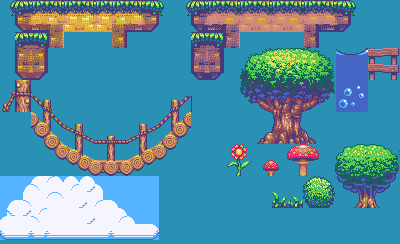
\includegraphics[scale = 1.0]{Imagens/tileset_edit.png}
    \caption{\textit{Exemplo de \textit{tileset}.}}
    \label{tileset_example}
\end{figure}
%
\par
%
O cenário final do jogo pode ser constituído de um único \textit{tiled layer} ou ser resultante da combinação 
de dois ou mais \textit{tiled layers}. Através da técnica de \textit{Tilemap}, torna-se possível construir inúmeros cenários,
com variadas dimensões, usando como base o mesmo \textit{tilesets}, aumentando a economia de memória e não reduzindo o desempenho no carregamento de imagens.
%
%
%
\begin{figure}[H]
    \centering
    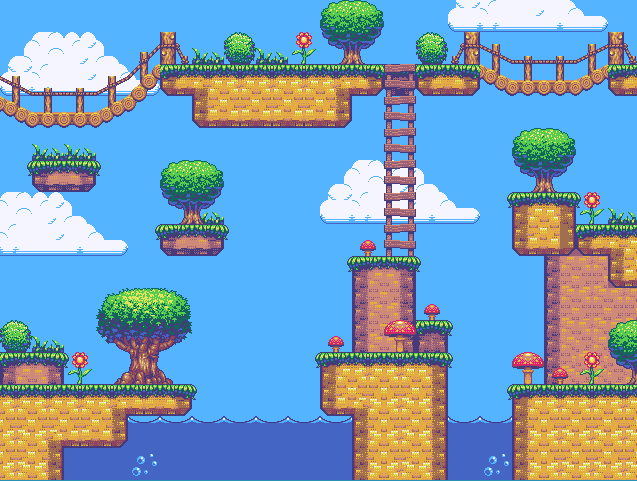
\includegraphics[scale = 0.65]{Imagens/cenario.png}
    \caption{\textit{Exemplo de um cenário construído com tileset.}}
    \label{cenario_example}
\end{figure}
%
%
\par
O software Tiled é uma ferramenta gratuita desenvolvida em C$++$ para a criação de layouts e mapas usando \textit{tilesets}
baseado na técnica de \textit{Tilemap}. De simples manuseio e grande versatilidade, o Tiled faz a edição de várias camadas de \textit{tiles} e salva tudo em um formato padronizado de extensão ``.tmx''. Uma das principais vantagens do formato TMX é sua organização, detalhamento e praticidade, sendo que seu conteúdo pode ser lido através do uso de um \textit{parser} para arquivos XML.
%
\begin{figure}[H]
    \centering
    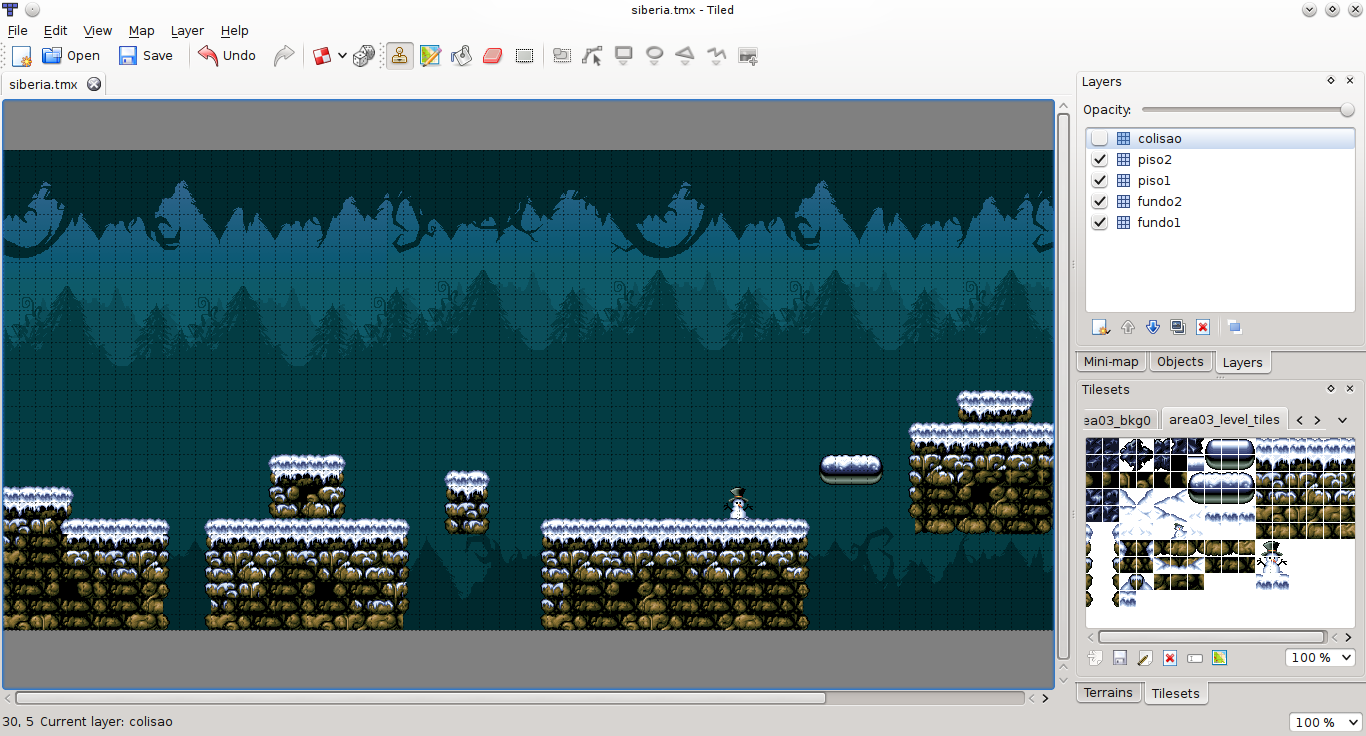
\includegraphics[scale = 0.45]{Imagens/Tiled.png}
    \caption{\textit{Interface do \textit{software} Tiled.}}
    \label{tiled_interface}
\end{figure}
%
\par
O Tiled é um editor de níveis que suporta mapas com projeções ortogonais e isométricas e ainda permite que 
objetos personalizados sejam salvos como imagens na resolução que desejar. Tem suporte também a comandos externos, 
plugins e formatos usados por outros editores. É compatível 
com diversas engines de criação de jogos e fornece meios de comprimir seus dados de modo a diminuir o tamanho em disco do arquivo TMX.
É possível, ainda, redimensionar e alterar o mapa posteriormente, criar múltiplos mapas em uma única sessão e ainda salvar ou 
restaurar até nove vezes. Com ele pode-se especificar o tamanho de cada tile em um \textit{tileset}, ou criar um mapa sem tamanho estrito 
sobre as imagens.
Mesmo que o desenvolvedor não queira que seu jogo seja baseado em \textit{tiles}, o software é ainda uma excelente escolha como um editor 
de níveis. Pode-se usá-lo também nas entidades invisíveis, tais como áreas de colisão e o aparecimento de objetos dentro do 
mapa. Por sua simplicidade não é necessário ter experiência em programação e até mesmo os não desenvolvedores podem usá-lo.
\par 
O processo de criação de um mapa com o Tiled é feito basicamente usando os passos abaixo:
%
\begin{enumerate}
 \item Escolher o tamanho do mapa e tamanho do tile base;
 \item Adicionar tilesets vindos de imagens;
 \item Adicionar quaisquer objetos que representem algo abstrato;
 \item Salvar o mapa no format TMX;
 \item Importar o arquivo TMX e interpretá-lo para o jogo.
\end{enumerate}
%%
O Tiled é totalmente gratuito. Esse detalhe aliado à sua facilidade de uso e versatilidade, tornaram-no extremamente popular em meio
a comunidade de desenvolvedores de jogos, onde não só estudantes e entusiastas, mas empresas e profissionais da área, passaram a adotá-lo 
como editor de níveis padrão. Seguindo esse pensamento, o nosso \textit{framework} a ser desenvolvido também possui suporte nativo
aos nveis contruídos usando este software.
%
\section{A biblioteca TinyXML}
\label{tinyXML}
%
É uma biblioteca escrita em C$++$ que analisa uma sequência de entrada no formato XML e cria uma estrutura independente 
de plataforma ou linguagem. Em outras palavras, ela realiza o \textit{parser} de uma arquivo .xml e armazena a informação 
em objetos C$++$ que podem ser manipulados livremente. 
\par 
A TinyXML pode ser facilmente integrada em outros programas, bastando apenas adicionar seus 
arquivos ao projeto. Com ela é possível realizar o acesso aos dados direta ou iterativamente, alteração da estrutura através 
de inserção e remoção de elementos, remoção de espaços duplicados e a gravação para ficheiros em formato XML.
TinyXML é uma estrutura extremamente compacta e robusta, elaborada para um rápido e fácil aprendizado. Pode ser usada para 
fins de código aberto ou comerciais. Ela é compatível com UTF-8, de modo a permitir que arquivos XML sejam manipulados em 
qualquer linguagem.
\par
No \textit{framework} que será desenvolvido, a TinyXML será responsável por realizar o \textit{parser} do arquivo .tmx gerado
pelo software Tiled.
%
%
%_____________________________________________________________________
% \chapter{Trabalho Desenvolvido}
% \label{cap:desenvolvido}
% 
% %_____________________________________________________________________
% \chapter{Conclusão}
% \label{cap:conclusao}
% 
% O objetivo principal deste trabalho foi consolidado pelo desenvolvimento....
% 
% %_____________________________________________________________________
% \section{Resultados}
% \label{sec:resultados}
% 
% A principal contribuição deste trabalho é a...
% 
% As contribuições secundárias deste trabalho pode-se citar:
% 
% \begin{itemize}
% \item contribuiçãoSecundária1
% \item contribuiçãoSecundária2
% \item contribuiçãoSecundária3
% \end{itemize}
% 
% %_____________________________________________________________________
% \section{Trabalhos Futuros}
% \label{sec:futuro}
% 
% Como continuidade desse trabalho, é possível citar como propostas:
% 
% \begin{itemize}
% \item trabalhoFuturo1
% \item trabalhoFuturo2
% \item trabalhoFuturo3
% \end{itemize}

%_________________________ Bibliografia _____________________________
\bibliographystyle{abntex2-alf} 
\bibliography{referencias}

\appendix
% \label{sec:anexos}
% 
% \chapter{Título do Apendice A}
% \lstinputlisting
% [
%    language=C++, 
%    label=code:hello, 
%    caption={Hello World}
% ]{hello.c}

\end{document}